\documentclass{acm_proc_article-sp}
\usepackage{float}
\begin{document}

\title{An introduction to Context-Oriented Programming}

\author{
\alignauthor
Ivo Willemsen\\
       \affaddr{Open Universiteit}\\
       \affaddr{Maastricht, The Netherlands}\\
       \email{ivo.willemsen@outlook.com}
}

\maketitle
\begin{abstract}
The last decade, use-cases have emerged that emphasize the need to cater to different behaviors depending on situation and context changes. Examples are pervasive systems and highly personalized business applications. Conventional programming languages offer constructs to implement context-dependent behavior, like  conditional branches such as if statements, but these branches often result in cluttered code and uses of those 
constructs seriously damage the modularity of the applications. In the early 2000s, a new programming paradigm emerged, called Context-Oriented Programming which intended to mitigate the aforementioned problems, by incorporating context as a part of the programming language, like variables, classes, and functions, etcetera. This paper presents an introduction to Context-Oriented Programming and explains how the concept of behavioral variations based on changing contexts can be exploited using Context-Oriented Programming languages.
\end{abstract}

\keywords{Context-Oriented Programming, context-aware systems, behavioral variations, layer activations} 

\section{Introduction} \label{introduction}
Many applications present behavior that is determined by the context in which it is being used. Examples of different contexts are: Battery level, GPS-location, available connectivity protocols (Wifi/3G/4G), speed of the network, user's preferences, etcetera.

For example, the battery level of a tablet or a smart phone on which an application (Operating System in this case) runs is a context. This context impacts many behavioral aspects of the application and it will not only have affect on the brightness of the screen, but it might also influence the way the Operating System prioritizes running threads and perhaps result in the preventive hibernation of the system.

In order to include context-dependent behavior in applications using most modern programming languages, one option available is to use the Strategy Design Pattern to abstract the context-dependent behavior into separate classes and decide at runtime-level which context-dependent behavior (strategy) to use. Another option would be the usage of conditional statements to find out the context in which a certain program is running. The usage of conditional statements in these cases would result in not adhering to one of the concepts of Object-Oriented Programming, namely to avoid conditional statements to determine polymorphic behavior. Both options are suboptimal as they result in cluttered code which is difficult to reuse and understand and which makes maintenance of the code a very cumbersome activity.

In many situations, behavioral variations are not implemented by a single object, rather it is spread over a group of cooperating objects. Functionality that is dispersed over several cooperating objects is called a crosscutting concern \cite{kiczalesetallaop}. Plain old Object-Oriented Programming languages don't have \textit{first-class constructs} that allow for modularization and composition of behavioral variations. A first-class construct \cite{Keays:2003:CP:940923.940926} is a construct which is an element of a language, like a class or a method in Java. 

The lack of aforementioned constructs in regular Object-Oriented Programming languages to support the development of context-aware applications, leaves the developer of those applications with the need to implement necessary \textit{boiler-plate code}. What is needed, is a type of language that incorporates those constructs; which allow a developer to focus more on the implementation of business use-cases and less on inventing the wheel of `context determination, modularization and activation` over and over again. 

The next section will zoom into the concept of `Context`, which contains basic Context-Oriented Programming jargon. The concepts that are explained in this section will be referred to in subsequent paragraphs. The concept of behavioral variations is introduced and an explanation is given on how to define behavioral variations in a class by using partial method definitions and layers. Finally, an elaboration is given of several types of behavioral variation activations.

\section{Context-Oriented Programming}
\label{cop}
In the early 2000s several approaches have been presented to support the development of context-aware applications. These approaches mainly encompass software architectures and component-based design \cite{SALVANESCHI20121801}. In 2008 the Context-Oriented Programming paradigm was proposed \cite{HirschfeldCostanzaNierstraszCOP} as a complementary approach for supporting dynamic adaptation to behavioral variations. 

This development was triggered by the appearance of a wide range of scenarios where applications had to react differently according to the active context. Conventional Object-Oriented Programming languages did not incorporate language structures that enabled developers to implement behavioral variations to changes in contexts in a modular way. 

Context-Oriented Programming promotes the modularization of context-dependent behavioral variations. It offers abstractions and mechanisms in the form of first-class constructs to define entities that need to change behavior depending on their context. It allows applications to be partitioned into behavioral variations that can be activated at runtime with predefined scopes. These behavioral variations are composed of \textit{partial definitions} for entities, like classes, functions, methods, procedures, etcetera. The essential ingredients of Context-oriented Programming \cite{Costanza:2008:CPC:1529966.1529970} are the following:

\begin{itemize}
\item {Context}
\item Behavioral variations
\item Layers
\item Layer activation
\item Scoping
\end{itemize}

\subsection{Context}
\label{sec:context}
Context can be defined as any information that can be used to characterize the situation of an entity. An entity is a person, place or object that is considered relevant to the interaction between a user and an application, including the user and the application themselves \cite{Abowd:1999:TBU:647985.743843}. Context is derived from three sources: Environment, system and the actors. Contextual information that originates from actors and the environment reaches the system from outside, but the system itself can also generate context. 

A \textit{system} is a set of computational objects, methods, functions that responds with predefined behavior on a per-request basis. An \textit{actor} is a person or another system that is directly involved with the system: It determines the order in which use-cases are executed by communicating directly with the system, by clicking on buttons, sending messages, receiving feedback, etcetera. An example of context generated by an actor is the choices made by a user when accessing certain functionalities that result in differences in behavior. Another example is the support of multiple devices (like an smart phone or a desktop computer) that add to the context-dependent behavior of the system. The \textit{environment} encompasses everything that lies outside the boundaries of the system, which is not directly involved in the relationship between the system and the actors.

Behavioral variations, changes in response, depend on the context that is generated by these three sources. As a result, context-dependent behavior variations can be split up into actor-dependent, environmental-dependent and  system-\linebreak dependent variations.

\textit{Context} is also commonly described as information that can be computationally accessed in a software system. This definition is kind of vague, as it leaves room for a variety of interpretations:

\begin{itemize}
\item The definition does not specify whether the information should originate from outside of the system, the environment, but it also comes from other sources like the actors and the system itself.
\item The granularity of abstraction is not enforced by the definition. Context can exist in the system, or can come to the system as fine-grained pieces of information, like indiscrete numerical temperature indications and can subsequently be transformed to more course-grained information classes like "low", "medium", "high". 
\item The uniqueness of the context is not imposed. There exist implementations of Context-Oriented Programming languages that enable applications to share only a common context. Other implementations don't follow this model and allow several contexts to exist, which are used in different parts of the application \cite{Appeltauer:2009:CCP:1562112.1562118}
\end{itemize}

\subsection{Behavioral variations}
\label{sec:behavioral_variations}
Context-Oriented Programming languages have first-class constructs that support \textit{behavioral variations} by means of partial definition of modules. Behavioral variations can be \textit{activated}, partly changing the behavior of the application. So, the function of behavior variations is to allow \textit{runtime activation} of a change in behavior and it also allows for the \textit{modularization} of behavior by exploiting the available constructs (by using layers) in the Context-Oriented Programming language.    

\subsection{Layers}
\label{sec:layers}
\textit{Layers} group context-dependent behavioral variations as first-class entities that can be explicitly referred to in a program at runtime. Layers are first-class entities in most Context-Oriented Programming languages, which group partial definitions and can be stored in variables and passed to methods. Several parts of the application can have access to the same layers and determine the exact changes in behavior that have to be done. In case of layers, the first-class entity that implements this functionality is a layered method. This method consists of a base, principle method definition, extended with at least one extra partial definition. This root layer which is always present, representing the base definition, defines the \textit{context-independent} behavior of the application.

The code snippets like the one in figure \ref{fig:layers} and in other figures in this paper, are based on the ContextJ implementation (Java-based) \cite{Appeltauer:2009:IDC:1562112.1562117}, but are by no means meant to be compile-ready as they only serve an explanatory goal. 

The use-case that is applicable should display client information with additional account and/or contact information, dependent on the kind of device that is used. Users that connect to the application through a smart phone, have less available real estate, so only basic client and account information is shown, whereas users that use a regular browser will have more space to show additional contact information, along with the client and account information. 

In figure \ref{fig:layers}, the base behavior of the ClientRepository (with no active layers), is to only retrieve the client information. The base definition of the get-method first checks the cache for the presence of the object that is associated with the id that is passed in. If found, it returns that object, if not found, it will get the object from the underlying data store, through the DAO-object (\textit{Data Access Object}). 

The get-method is partially redefined in two layers that are defined in the same class by making use of the first-class construct "layer". In case the mobile layer is active, first the base functionality of the get-method will be invoked by the proceed-call. After the proceed-call has retrieved the object, the partial definition will make a call to the DAO object in order to retrieve the account information that is related with the client. Before returning the object to the caller, the partial definition will make sure that the cache is updated with the newly retrieved information. 
\begin{figure}[H]
\centering
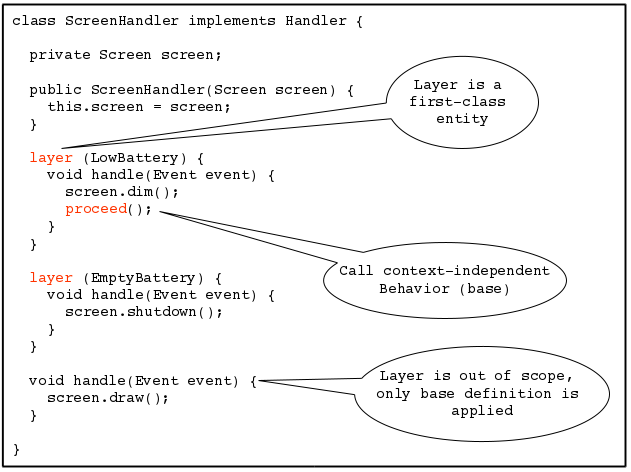
\includegraphics[width=90mm]{layers_toy.png}
\caption{Layers, behavioral variations and base/partial definition}
\label{fig:layers}
\end{figure}
So, based on the use-case, account and/or contact information can be \textit{lazily loaded}, by activating the corresponding layers, achieving a simple context-dependent and performance-wise efficient solution. Of course, the above use-case and sample implementation is a very simplified abstraction of what could be a real solution, depending on defined functional and non-functional requirements.

The \textit{layer modularization technique }that has been used to allocate layers in figure \ref{fig:layers}, is called the \textit{layers-in-class} style allocation. On a per-class basis, layers are defined. This means that layer definitions are \textit{scattered} over all the classes to which a certain behavioral variation should be applied. When there exist too many classes to which a certain behavioral variation must be applied, there is another technique to avoid the aforementioned problem, which is called \textit{class-in-layer} allocation of layers. The most optimal choice depends on the number of behavioral variations and classes.

\subsection{Layer activation and scoping}
\label{sec:layer_activation_scoping}
The main reason for the existence of Context-Oriented Programming languages is the need to dynamically adapt to different behavioral variations in an elegant and modular way, so this paradigm must provide for regularly changing application behavior. The concept of changing  application behavior is implemented by activating and deactivating layers at a certain point in time during the execution of the application. \textit{Layer activation} is achieved by language constructs that ensure that layers are added at runtime, such that certain partial method definitions have an influence on the actual behavior of an application \cite{Kamina:2014:CSE:2577080.2579816}. 

By default, only the root layer is active at runtime. So only the base definition associated with the root layer will directly influence the behavior of the application. Other layers can be activated and deactivated by using specific keywords that have been added to the programming language or the extension. 

The following subparagraphs will shed a light on the different activation mechanisms that have been described in implementation proposals or are available in implementations. It needs to be said that regarding this subject, there is no consensus among either the Context-Oriented Programming language that have been developed or many specifications for Context-Oriented Programming languages that have been published throughout the years. Layer activation and deactivation mechanisms are a complex matter and the most suited approach depends a lot on the architecture and the proposed use-case of the Context-Oriented Programming language.

\subsubsection{Dynamically scoped activation}
\label{dynamically_scoped_activation}
Most Context-Oriented Programming languages support the use of \textit{dynamically scoped activation}. A series of layers can be activated by the use of the keyword "with". Multiple uses of with-statements in nested calls will add the specified layer to the configuration of layers that are active at that point. The scope of a set of certain active layers is determined by the with-block. At the moment that a with-block terminates, the scope expires and affected layers are removed (\textit{implicit deactivation}) from the configuration of active layers. 

\begin{figure}[H]
\centering
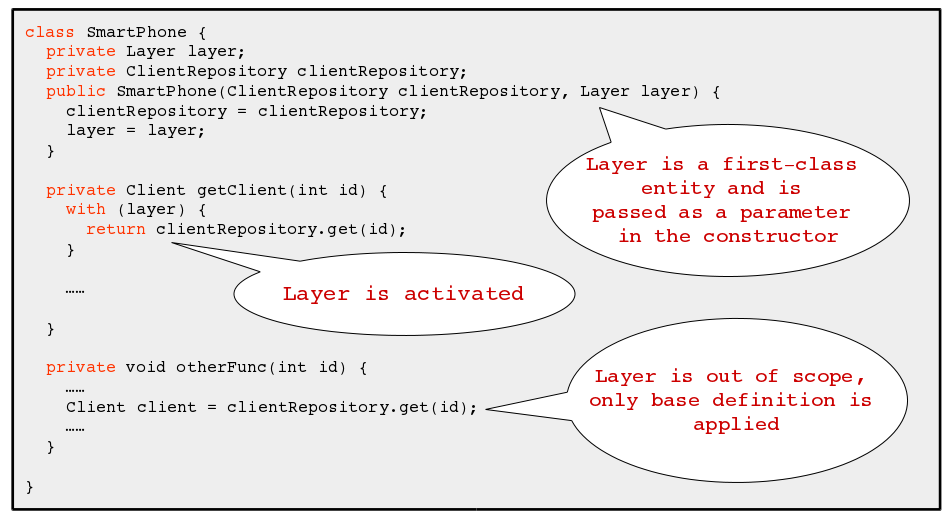
\includegraphics[width=85mm]{dynamic_activation2.png}
\caption{Dynamically scoped activation}
\label{fig:dynamically_scoped_activation}
\end{figure}

The concept of \textit{dynamically scoped activation}, or \textit{direct layer activation}, is depicted in figure \ref{fig:dynamically_scoped_activation}. When the SmartPhone class is constructed, the appropriate layer is provided as part of one of the constructor parameters. In the case of a smart phone, the most probable behavior that would be linked with the display properties of the device is to be as efficient as possible with the amount of information that is provided, thus choosing the mobileLayer. When the call is made to the ClientRepository to retrieve the client information, the appropriate logic that belongs to the mobileLayer is executed after the base definition has been applied. As a result, only client and account information is displayed on the SmartPhone. 

After the with-block has terminated, the mobileLayer layer is out-of-scope, and subsequent similar calls to the Client-Repository to retrieve the client information, will result in the retrieval of only the basic client information, without account or contact information.

\subsubsection{Indefinite activation}
\label{indefinite_activation}
Dynamically scoped activation is the preferred mechanism of activation of layers in case of functional behavioral adaption. Situations exists where certain non-functional crosscutting aspects need to be weaved into the application as part of an initial configuration setup. Initially they are applied when probably the applications starts up, and changes to the configuration of active layers are not made during the rest of the execution flow. An example is the incorporation of a logging facility, where a system can be started in debug mode in case issues arise in a production environment. After the production outage has been solved, the system's logging option can be reset and the system can be brought up again in normal mode. To facilitate this, \textit{static layer activation} or \textit{indefinite activation} can be applied  \cite{SALVANESCHI20121801}. Note that using indefinite activation implies that there are no scope restriction: All classes that have behavioral variations are affected by the layers that are being configured. 

A variation to indefinite activation, is implicit activation. Like, indefinite activation, implicit activation influences all the classes without scope restriction, but in the latter case, an explicit configuration of the active layers is done during the execution of the flow. 

\subsubsection{Per-object activation}
\label{per_object_activation}
This type of activation allows configuration of active layers to be performed on single instances of classes. It can be used as an "add-on" and usually it is applied in combination with dynamically scoped activation. In cases where, on top of applying a  globally scoped activation of behavior, it is also necessary to apply a certain behavioral variation on a small subset of instances of classes, explicit setting the appropriate layer on the instance-level can be done \cite{SALVANESCHI20121801}. Figure \ref{fig:per_object_activation} illustrates the concept of per-object activation.

\begin{figure}[H]
\centering
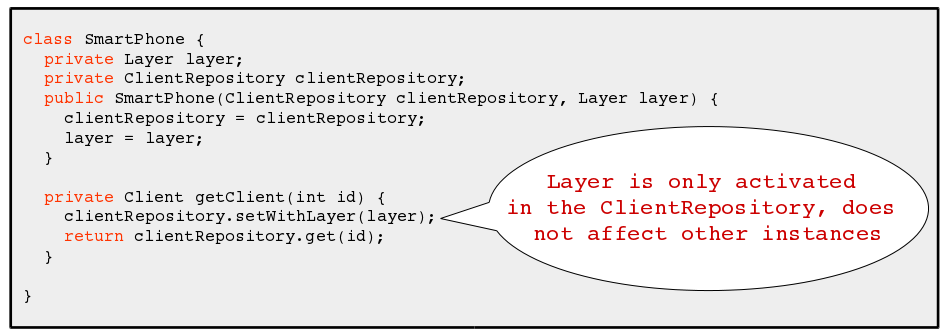
\includegraphics[width=85mm]{per_object_activation2.png}
\caption{Per-object activation}
\label{fig:per_object_activation}
\end{figure}

\section{Further reading}
\label{sec:further_reading}
This paper gives an introduction to Context-Oriented Programming. A next step could be to get more information regarding Context-Oriented Software Architecture \cite{Mens:2016:CSA:2951965.2951971}. Also sources are available that discuss Context-Oriented Programming in a more detailed fashion, explaining more about activation mechanisms, design patters and modularization \cite{SALVANESCHI20121801}. This paper does not discuss an implementation, there are papers available that elaborate more on real implementations, like the ContextJ implementation for Java \cite{Appeltauer:2009:IDC:1562112.1562117}. 

\section{Conclusion}
\label{sec:conclusion}
The purpose of this paper was to introduce novices to Context-Oriented Programming and explain how applications developed with Context-Oriented Programming languages implement behavioral variations based on changing contexts. 

A simple hypothetical use-case has been presented and a simplified Context-Oriented Programming language, based on ConttextJ, with a reduced subset of functionalities was used to show how layers, that encapsulate behavioral variations, can be defined. Several types of activation mechanisms were presented that can be used in order to link behavioral variations based on context changes. 

\bibliographystyle{abbrv}
\bibliography{essence_of_cop}
\end{document}
